\section{The gain persists with more data and greater width}
\label{sec:scaling}

WT-MLP-Lag lowers final loss relative to MuonT in all three training regimes. The improvement is small in absolute units, but adds 29--43\% to the held-out gain that input preconditioning already obtains over Muon. For held-out loss, the relative extension is $(\mathcal L_{\rm MuonT}-\mathcal L_{\rm WT})/(\mathcal L_{\rm Muon}-\mathcal L_{\rm MuonT})$. Its denominator is 0.0119, 0.0103, and 0.0065 nats in the three regimes. The direct differences in \Cref{tab:main_scaling} show the effect size and replication level.

\begin{table}[!htb]\centering\small
\setlength{\tabcolsep}{2.2pt}
\caption{\textbf{Confirmatory and scaling results across fresh seeds, longer horizon, and greater width.} Held-out reports final cross-entropy $\Lsel$ in nats; all $\Delta$ columns report differences from same-regime Muon in millinats (negative favors the row method). MuonT applies input preconditioning only, so the gap between the MuonT and WT-MLP-Lag rows isolates the output-side contribution. Late-11 averages the 11 second-half checkpoints; Wins counts the 16 Paloma domains improved over Muon. At 130M, all four methods share their bracketed seed-0 optimum ($\eta^*=0.01600$ at 20 TPP and $0.01600\times4^{-0.3}=0.01056$ at 80 TPP); at 520M Muon runs at its own selected rate while the preconditioned methods share MuonT's pinned rate, so that block compares each method at its chosen rate rather than at a matched one. Complete absolute losses and $\eta=0.02263$ replicates appear in \Cref{tab:absolute_results,tab:seeds}.}\label{tab:main_scaling}
\begin{tabularx}{\textwidth}{@{}>{\raggedright\arraybackslash}Xrrrrrrr@{}}
\toprule
& & (nats) & \multicolumn{4}{c}{Differences from Muon (millinats, $\downarrow$)} & Paloma \\
\cmidrule(lr){4-7}
Method & LR $\eta$ & Held-out & $\Delta$ Held-out & Late-11 $\Delta$ & $\Delta$ C4 & $\Delta$ Paloma & Wins \\
\midrule
\addlinespace[2pt]\multicolumn{8}{@{}l}{\textit{130M confirmation: 20 TPP, 2.68B tokens, fresh seeds 1--3 (matched $\eta^*=0.0160$, paired mean $\pm$ SD)}}\\
Muon & 0.01600 & 3.2035 & $+0.00$ & $+0.00$ & $+0.00$ & $+0.00$ & --- \\
MuonT & 0.01600 & 3.1916 & $-11.91\pm1.40$ & $-23.26\pm2.07$ & $-11.79\pm0.98$ & $-11.49\pm4.18$ & 16/16 \\
OD-All & 0.01600 & 3.1919 & $-11.62\pm1.09$ & $-22.91\pm1.63$ & $-12.63\pm1.22$ & $-12.79\pm1.92$ & 16/16 \\
\rowcolor{rowtint}[0pt][0pt]\textbf{WT-MLP-Lag} & 0.01600 & \textbf{3.1881} & $\mathbf{-15.41\pm2.18}$ & $\mathbf{-26.78\pm2.30}$ & $\mathbf{-15.64\pm1.80}$ & $\mathbf{-15.91\pm1.68}$ & \textbf{16/16} \\
\addlinespace[5pt]\multicolumn{8}{@{}l}{\textit{130M longer training: 80 TPP, 10.74B tokens, seed 0 (matched rate)}}\\
Muon & 0.01056 & 3.0778 & $+0.00$ & $+0.00$ & $+0.00$ & $+0.00$ & --- \\
MuonT & 0.01056 & 3.0675 & $-10.28$ & $-22.28$ & $-10.26$ & $-11.12$ & 15/16 \\
OD-All & 0.01056 & 3.0656 & $-12.19$ & $-23.85$ & $-12.82$ & $-13.71$ & 16/16 \\
\rowcolor{rowtint}[0pt][0pt]\textbf{WT-MLP-Lag} & 0.01056 & \textbf{3.0636} & $\mathbf{-14.23}$ & $\mathbf{-26.82}$ & $\mathbf{-14.07}$ & $\mathbf{-16.78}$ & \textbf{16/16} \\
\addlinespace[5pt]\multicolumn{8}{@{}l}{\textit{520M width transfer: 20 TPP, 10.74B tokens, $\dm=1{,}024$, seed 0 (pinned rate)}}\\
Muon & 0.01600 & 2.8528 & $+0.00$ & $+0.00$ & $+0.00$ & $+0.00$ & --- \\
MuonT & 0.02263 & 2.8463 & $-6.45$ & $-1.87$ & $-6.49$ & $-3.49$ & 15/16 \\
OD-All & 0.02263 & 2.8469 & $-5.88$ & $-1.28$ & $-6.09$ & $-3.02$ & 14/16 \\
\rowcolor{rowtint}[0pt][0pt]\textbf{WT-MLP-Lag} & 0.02263 & \textbf{2.8435} & $\mathbf{-9.25}$ & $\mathbf{-4.92}$ & $\mathbf{-8.71}$ & $\mathbf{-8.93}$ & \textbf{15/16} \\
\bottomrule\end{tabularx}
\end{table}


\subsection{Fresh seeds confirm an incremental benefit}
\label{sec:phase2}

On fresh 130M seeds 1--3 at the shared full-budget optimum $\eta^*=0.016$, WT-MLP-Lag improves on MuonT on every seed across held-out mixture, C4, and Paloma macro loss, as well as across late-training checkpoints (\Cref{tab:main_scaling}). Its paired held-out improvement is $0.0035\pm0.0017$ nats (mean $\pm$ sample standard deviation across seeds), whereas OD-All leaves held-out mixture loss essentially unchanged ($+0.0003\pm0.0004$ nats). Repeating both output methods on the same seeds at $\eta=0.02263$ yields the same ranking ($0.0034\pm0.0015$ versus $0.0005\pm0.0005$ nats; \Cref{tab:absolute_results,tab:seeds}). Retaining cross-channel correlations at hidden width therefore accounts for the 130M gain rather than learning-rate selection or coordinate scaling alone.

The improvement also survives a doubled global batch of 1M tokens: the checked run gains 0.0036 nats on held-out mixture and 0.0040 nats on C4 relative to MuonT. This is a batch-size check, not an additional multi-seed confirmation.

\subsection{Longer training retains the gain at matched learning rates}
\label{sec:phase3}

Training 130M for 10.74B tokens tests whether MuonT catches up once the token budget grows fourfold. At a shared learning rate of 0.01056, WT-MLP-Lag finishes 0.0040 nats lower on held-out mixture and stays ahead at every second-half checkpoint. Its Paloma macro gain is 0.0057 nats, with improvements on all 16 domains. The fixed-token advantage therefore persists through the 80-TPP schedule in this seed.

The shared rate $\eta=0.016\times4^{-0.3}=0.01056$ scales the common 20-TPP optimum to the fourfold horizon. Scaling from the hotter $\eta=0.02263$ grid point instead ($\eta=0.01493$, $\sqrt2\times$ higher) develops a mid-training penalty and finishes worse on Paloma (\Cref{fig:scaling_traj}(b),\Cref{tab:absolute_results}). A useful output approximation therefore does not remove sensitivity to horizon-scaled learning rates.

\begin{figure}[t]
 \centering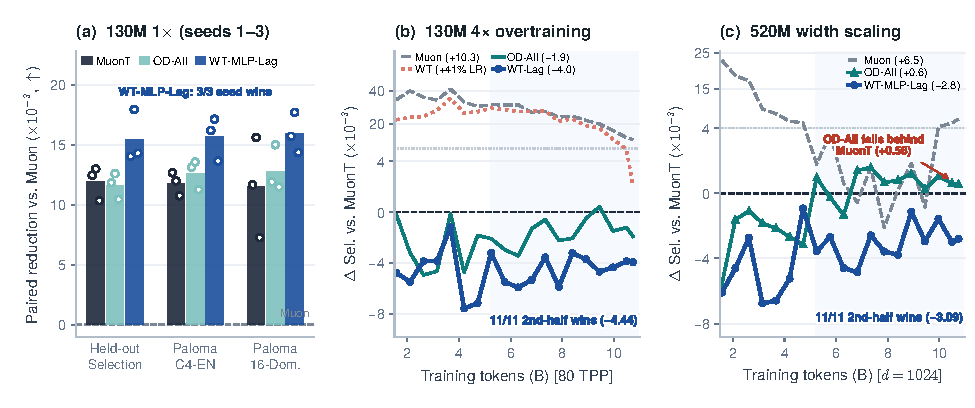
\includegraphics[width=\textwidth]{fig5_scaling_trajectories.pdf}
 \caption{\textbf{The width-thresholded gain survives fresh seeds, longer training, and greater width.}
 \textbf{(a)} Final loss reductions versus same-seed Muon at 130M, 20 TPP. Bars show three-seed means; open circles show individual seeds.
 \textbf{(b, c)} Held-out differences from MuonT during the 10.74B-token runs: 130M at 80 TPP and 520M at 20 TPP, each with one seed. The hotter WT run in (b) shows learning-rate sensitivity. Vertical axes compress the positive range above the dotted lines; negative differences indicate lower loss.}
 \label{fig:scaling_traj}
\end{figure}

\subsection{Wider models expose the limit of all-diagonal outputs}
\label{sec:phase4}

Doubling hidden width to 1,024 separates the two output approximations. OD-All finishes slightly worse than MuonT on held-out mixture, C4, and Paloma macro loss. WT-MLP-Lag instead improves held-out loss by 0.0028 nats and remains ahead at all 11 late checkpoints. All three preconditioned methods use MuonT's pinned 520M rate of 0.02263, with no output-side retuning.

The out-of-distribution evaluation supports the same distinction. WT-MLP-Lag improves on MuonT in 15 of 16 Paloma domains; OD-All improves in six. The domain plot exposes both the spread of gains and the remaining regression instead of relying only on a macro average (\Cref{fig:paloma}). Since domains share training and evaluation influences, these win counts describe coverage rather than independent replications.

\begin{figure}[t]
 \centering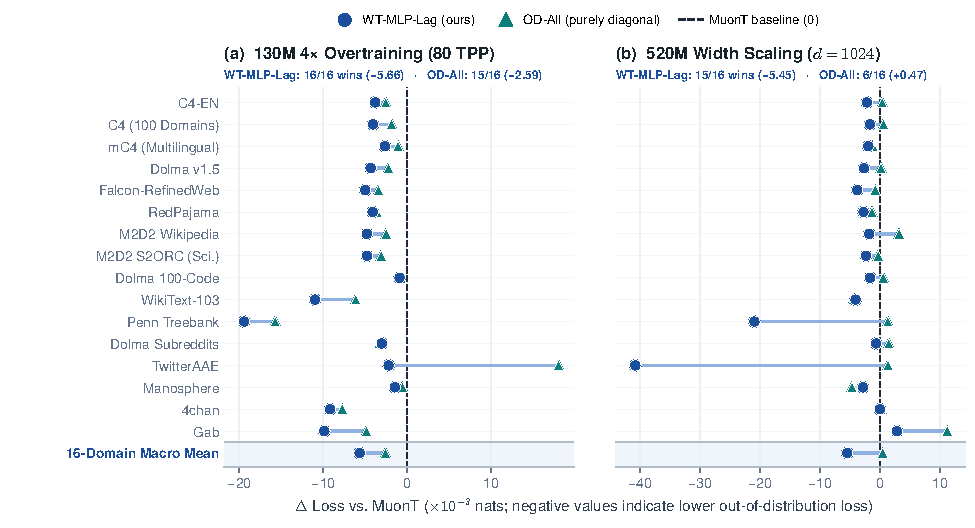
\includegraphics[width=\textwidth]{fig6_paloma_domains.pdf}
 \caption{\textbf{Most Paloma domains benefit from retaining dense hidden-width outputs.}
 Final per-domain loss differences from MuonT. \textbf{(a)} At 130M, 80 TPP, WT-MLP-Lag wins 16/16 domains. \textbf{(b)} At 520M, 20 TPP, it wins 15/16 and OD-All wins 6/16. Circles denote WT-MLP-Lag; triangles denote OD-All. The bottom row gives the unweighted macro mean. Panels use different horizontal scales; connecting lines compare methods within a domain and are not confidence intervals. Each regime uses one seed.}
 \label{fig:paloma}
\end{figure}

Two widths do not establish an asymptotic scaling law. We next test the proposed directional explanation on saved checkpoints.
